%---------------------------------------------------------------------------%
%-                                                                         -%
%-                           LaTeX Template                                -%
%-                                                                         -%
%---------------------------------------------------------------------------%
%- Copyright (C) Huangrui Mo <huangrui.mo@gmail.com>
%- This is free software: you can redistribute it and/or modify it
%- under the terms of the GNU General Public License as published by
%- the Free Software Foundation, either version 3 of the License, or
%- (at your option) any later version.
%---------------------------------------------------------------------------%
%->> Document class declaration
%---------------------------------------------------------------------------%
\documentclass[singlesided]{Style/ucasthesis}%
%- Multiple optional arguments:
%- [<singlesided|doublesided|printcopy>]% set one or two sided eprint or print
%- [draftversion]% show draft version information
%- [fontset=<fandol|...>]% specify font set to replace automatic detection
%- [scheme=plain]% thesis writing of international students
%- [standard options for ctex book class: draft|paper size|font size|...]%
%---------------------------------------------------------------------------%
%->> Document settings
%---------------------------------------------------------------------------%
\usepackage[authoryear,myhdr,list]{Style/artratex}% document settings
%- usage: \usepackage[option1,option2,...,optionN]{artratex}
%- Multiple optional arguments:
%- [bibtex|biber]% set bibliography processor and package
%- [<numbers|super|authoryear|alpha>]% set citation and reference style
%- <numbers>: textual: Jones [1]; parenthetical: [1]
%- <super>: textual: Jones superscript [1]; parenthetical: superscript [1]
%- <authoryear>: textual: Jones (1995); parenthetical: (Jones, 1995)
%- <alpha>: textual: not available; parenthetical: [Jon95]
%- [geometry]% reconfigure page layout via geometry package
%- [lscape]% provide landscape layout environment
%- [myhdr]% enable header and footer via fancyhdr package
%- [color]% provide color support via xcolor package
%- [background]% enable page background
%- [tikz]% provide complex diagrams via tikz package
%- [table]% provide complex tables via ctable package
%- [list]% provide enhanced list environments for algorithm and coding
%- [math]% enable some extra math packages
\usepackage{Style/artracom}% user defined commands

%%%%%%%%%%%%%%
\usepackage{fancyvrb}
\usepackage{hologo}

% \setlength{\hfuzz}{3pt}
% \ctexset{linestretch = 2\ccwd}
% \setlength{\bibitemsep}{3bp}
% \renewcommand*{\bibfont}{\zihao{5}\linespread{1.27}\selectfont}

\hypersetup{colorlinks = true, allcolors = blue}
\newcommand{\myemph}[1]{\emph{\textcolor{red}{#1}}}
\newcommand{\unemph}[1]{\textup{\textcolor{black}{#1}}}
\newcommand{\docversion}{v1.7.4}

\usepackage{longtable,booktabs}

\usepackage{amssymb,amsmath}
%\usepackage{natbib}
%\bibliographystyle{apalike}
\newcommand{\VerbBar}{|}
\newcommand{\VERB}{\Verb[commandchars=\\\{\}]}
\DefineVerbatimEnvironment{Highlighting}{Verbatim}{commandchars=\\\{\}}
% Add ',fontsize=\small' for more characters per line
\usepackage{framed}
\definecolor{shadecolor}{RGB}{248,248,248}
\newenvironment{Shaded}{\begin{snugshade}}{\end{snugshade}}
\newcommand{\KeywordTok}[1]{\textcolor[rgb]{0.13,0.29,0.53}{\textbf{{#1}}}}
\newcommand{\DataTypeTok}[1]{\textcolor[rgb]{0.13,0.29,0.53}{{#1}}}
\newcommand{\DecValTok}[1]{\textcolor[rgb]{0.00,0.00,0.81}{{#1}}}
\newcommand{\BaseNTok}[1]{\textcolor[rgb]{0.00,0.00,0.81}{{#1}}}
\newcommand{\FloatTok}[1]{\textcolor[rgb]{0.00,0.00,0.81}{{#1}}}
\newcommand{\ConstantTok}[1]{\textcolor[rgb]{0.00,0.00,0.00}{{#1}}}
\newcommand{\CharTok}[1]{\textcolor[rgb]{0.31,0.60,0.02}{{#1}}}
\newcommand{\SpecialCharTok}[1]{\textcolor[rgb]{0.00,0.00,0.00}{{#1}}}
\newcommand{\StringTok}[1]{\textcolor[rgb]{0.31,0.60,0.02}{{#1}}}
\newcommand{\VerbatimStringTok}[1]{\textcolor[rgb]{0.31,0.60,0.02}{{#1}}}
\newcommand{\SpecialStringTok}[1]{\textcolor[rgb]{0.31,0.60,0.02}{{#1}}}
\newcommand{\ImportTok}[1]{{#1}}
\newcommand{\CommentTok}[1]{\textcolor[rgb]{0.56,0.35,0.01}{\textit{{#1}}}}
\newcommand{\DocumentationTok}[1]{\textcolor[rgb]{0.56,0.35,0.01}{\textbf{\textit{{#1}}}}}
\newcommand{\AnnotationTok}[1]{\textcolor[rgb]{0.56,0.35,0.01}{\textbf{\textit{{#1}}}}}
\newcommand{\CommentVarTok}[1]{\textcolor[rgb]{0.56,0.35,0.01}{\textbf{\textit{{#1}}}}}
\newcommand{\OtherTok}[1]{\textcolor[rgb]{0.56,0.35,0.01}{{#1}}}
\newcommand{\FunctionTok}[1]{\textcolor[rgb]{0.00,0.00,0.00}{{#1}}}
\newcommand{\VariableTok}[1]{\textcolor[rgb]{0.00,0.00,0.00}{{#1}}}
\newcommand{\ControlFlowTok}[1]{\textcolor[rgb]{0.13,0.29,0.53}{\textbf{{#1}}}}
\newcommand{\OperatorTok}[1]{\textcolor[rgb]{0.81,0.36,0.00}{\textbf{{#1}}}}
\newcommand{\BuiltInTok}[1]{{#1}}
\newcommand{\ExtensionTok}[1]{{#1}}
\newcommand{\PreprocessorTok}[1]{\textcolor[rgb]{0.56,0.35,0.01}{\textit{{#1}}}}
\newcommand{\AttributeTok}[1]{\textcolor[rgb]{0.77,0.63,0.00}{{#1}}}
\newcommand{\RegionMarkerTok}[1]{{#1}}
\newcommand{\InformationTok}[1]{\textcolor[rgb]{0.56,0.35,0.01}{\textbf{\textit{{#1}}}}}
\newcommand{\WarningTok}[1]{\textcolor[rgb]{0.56,0.35,0.01}{\textbf{\textit{{#1}}}}}
\newcommand{\AlertTok}[1]{\textcolor[rgb]{0.94,0.16,0.16}{{#1}}}
\newcommand{\ErrorTok}[1]{\textcolor[rgb]{0.64,0.00,0.00}{\textbf{{#1}}}}
\newcommand{\NormalTok}[1]{{#1}}
%%%%%%%%%%%%%%


%---------------------------------------------------------------------------%
%->> Document inclusion
%---------------------------------------------------------------------------%
%\includeonly{Tex/Chap_1,...,Tex/Chap_N}% selected files compilation
%---------------------------------------------------------------------------%
%->> Document content
%---------------------------------------------------------------------------%
\begin{document}
%-
%-> Frontmatter: title page, abstract, content list, symbol list, preface
%-
\frontmatter% initialize the environment

%---------------------------------------------------------------------------%
%->> 封面信息及生成
%---------------------------------------------------------------------------%
%-
%-> 中文封面信息
%-
\confidential{}% 密级:只有涉密论文才填写
\schoollogo{scale=0.5}{zuel_logo}% 校徽
\title{中南财经政法大学本科生学位论文 bookdown 模板(非官方)}% 论文中文题目
\author{donk3yzz}% 论文作者
\advisor{谷哥教授}% 指导教师:姓名 专业技术职务 工作单位
\advisorsec{}% 指导老师附加信息 或 第二指导老师信息
\degree{学士}% 学位:学士、硕士、博士
\degreetype{理学}% 学位类别:理学、工学、工程、医学等
\major{论文排版}% 二级学科专业名称
\institute{R 语言学院}% 院系名称
\chinesedate{2018 年 9 月}% 毕业日期:夏季为6月、冬季为12月
%-
%-> 英文封面信息
%-
\englishtitle{Zhongnan University of Economics and Law undergraduate graduation thesis template}% 论文英文题目
\englishauthor{Feng, Shengshi}% 论文作者
\englishadvisor{Supervisor: Prof.Google}% 指导教师
\englishdegree{Master}% 学位:Bachelor, Master, Doctor。封面格式将根据英文学位名称自动切换,请确保拼写准确无误
\englishdegreetype{Natural Science}% 学位类别:Philosophy, Natural Science, Engineering, Economics, Agriculture 等
\englishthesistype{thesis}% 论文类型: thesis, dissertation
\englishmajor{Typesetting}% 二级学科专业名称
\englishinstitute{College of R}% 院系名称
\englishdate{September, 2018}% 毕业日期:夏季为June、冬季为December
%-
%-> 生成封面
%-
\maketitle% 生成中文封面
%\makeenglishtitle% 生成英文封面
%-
%-> 作者声明
%-
%
%
\makedeclaration% 生成声明页
\makezueltitle% 生成中南财经政法大学论文标题面
%-
%-> 中文摘要
%-
\setcounter{page}{1}% 开始页码
\pagenumbering{arabic}% 页码符号
\chapter{摘要}%\chaptermark{摘\quad要}% 摘要标题
这里写中文摘要。啊不可挡家真的好。测试测试测试测试测试测试测试测试测试测试测试测试测试测试测试测试测试测试
%\keywords{排版,文档类}% 中文关键词

\cabstract{这里写中文摘要。啊不可挡家真的好。测试测试测试测试测试测试测试测试测试测试测试测试测试测试测试测试测试测试}{排版,文档类}
%-
%-> 英文摘要
%-
\chapter*{Abstract} %\chaptermark{Abstract}% 摘要标题
%

\englishkeywords{\hologo{LaTeX2e}, \CTeX{}, bookdown}% 英文关键词
%---------------------------------------------------------------------------%



{% content list region
\linespread{1.2}% local line space
%\intotoc{\contentsname}% add link to contents table and bookmark
\tableofcontents% contents catalog
%\intotoc{\listfigurename}% add link to contents table and bookmark
\listoffigures% figures catalog
%\intotoc{\listtablename}% add link to contents table and bookmark
\listoftables% tables catalog
}
\chapter*{符号列表}
\chaptermark{符号列表}

\section*{字符}
\nomenclatureitem[\textbf{Unit}]{\textbf{Symbol}}{\textbf{Description}}
\nomenclatureitem[$\Unit{m^{2} \cdot s^{-2} \cdot K^{-1}}$]{$R$}{the gas constant}
\nomenclatureitem[$\Unit{m^{2} \cdot s^{-2} \cdot K^{-1}}$]{$C_v$}{specific heat capacity at constant volume}
\nomenclatureitem[$\Unit{m^{2} \cdot s^{-2} \cdot K^{-1}}$]{$C_p$}{specific heat capacity at constant pressure}
\nomenclatureitem[$\Unit{m^{2} \cdot s^{-2}}$]{$E$}{specific total energy}
\nomenclatureitem[$\Unit{m^{2} \cdot s^{-2}}$]{$e$}{specific internal energy}
\nomenclatureitem[$\Unit{m^{2} \cdot s^{-2}}$]{$h_T$}{specific total enthalpy}
\nomenclatureitem[$\Unit{m^{2} \cdot s^{-2}}$]{$h$}{specific enthalpy}
\nomenclatureitem[$\Unit{kg \cdot m \cdot s^{-3} \cdot K^{-1}}$]{$k$}{thermal conductivity}
\nomenclatureitem[$\Unit{kg \cdot m^{-1} \cdot s^{-2}}$]{$S_{ij}$}{deviatoric stress tensor}
\nomenclatureitem[$\Unit{kg \cdot m^{-1} \cdot s^{-2}}$]{$\tau_{ij}$}{viscous stress tensor}
\nomenclatureitem[$\Unit{1}$]{$\delta_{ij}$}{Kronecker tensor}
\nomenclatureitem[$\Unit{1}$]{$I_{ij}$}{identity tensor}

\section*{算子}
\nomenclatureitem{\textbf{Symbol}}{\textbf{Description}}
\nomenclatureitem{$\Delta$}{difference}
\nomenclatureitem{$\nabla$}{gradient operator}
\nomenclatureitem{$\delta^{\pm}$}{upwind-biased interpolation scheme}

\section*{缩写}
\nomenclatureitem{CFD}{Computational Fluid Dynamics}
\nomenclatureitem{CFL}{Courant-Friedrichs-Lewy}
\nomenclatureitem{EOS}{Equation of State}
\nomenclatureitem{JWL}{Jones-Wilkins-Lee}
\nomenclatureitem{WENO}{Weighted Essentially Non-oscillatory}
\nomenclatureitem{ZND}{Zel'dovich-von Neumann-Doering}

% list of symbols, preface content
%-
%-> Mainmatter
%-

\setcounter{page}{1}
\mainmatter% initialize the environment
\mainmatter

\hypertarget{section}{%
\chapter{引言}\label{section}}

很高兴地宣布,我的 R 语言扩展包 `bookdownplus' (Zhao \protect\hyperlink{ref-R-bookdownplus}{2017}) 在 CRAN 正式发布了。

bookdownplus 是对 bookdown 包 (Xie \protect\hyperlink{ref-R-bookdown}{2016}) 的增强和简化。bookdown 就好比 Microsoft Word 或 LaTeX,可以用来写文档,而 bookdownplus 提供了很多有用的模板,可以很方便地在 bookdown 平台写期刊论文、学位论文、学术海报、化学分子式、信件、日记、日历、诗集、吉他谱等各种常用文档和书籍。这是功能上的增强(+)。

bookdownplus 使用时只需指定一个模板,给定作者和书名,就可以一键生成模板文件,用户在模板文件里照猫画虎写自己的文字就可以了,不必再花力气上网找模板、设置 YAML 和 LaTeX。这是操作上的简化(-)。

bookdownplus 各个模板的使用方法详见 \href{https://bookdown.org/baydap/bookdownplus}{R bookdownplus Textbook}。这本电子书本身就是用 bookdownplus 生成的,尤其是它的 \href{https://bookdown.org/baydap/bookdownplus/bookdownplus.pdf}{pdf 版本}很美观。此书的源码开放,可以作为使用 bookdownplus写书的示例。

\begin{figure}

{\centering 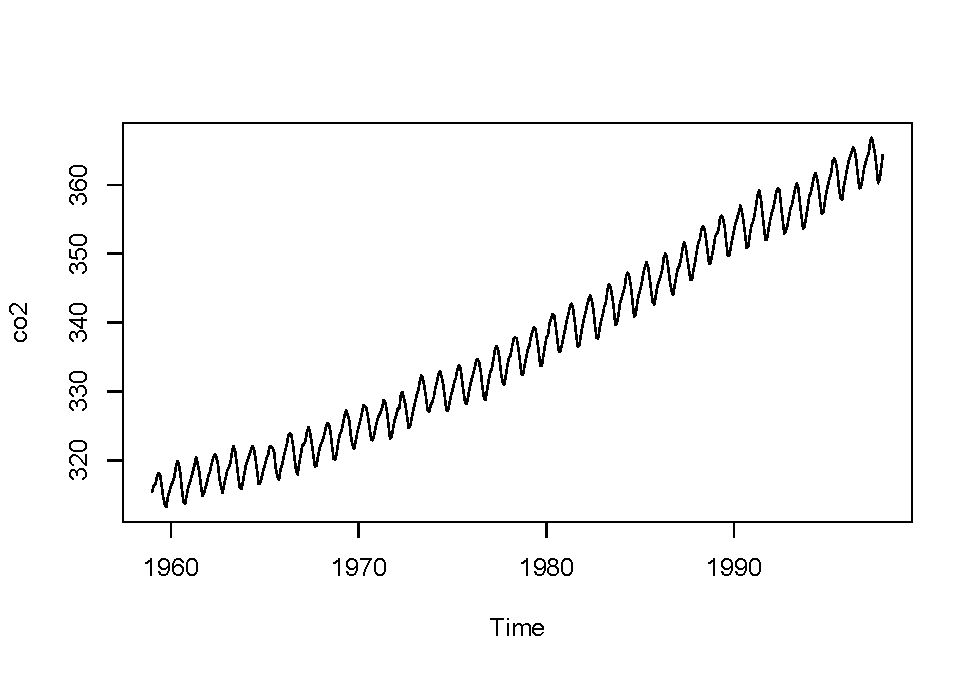
\includegraphics[width=0.8\linewidth]{ucas_zh_files/figure-latex/co2-1} 

}

\caption{用 R 语言画个图试试}\label{fig:co2}
\end{figure}

图 \ref{fig:co2} 是 CO\textsubscript{2} 数据。

表 \ref{tab:tabair} 是空气质量数据。

\begin{Shaded}
\begin{Highlighting}[]
\NormalTok{knitr}\OperatorTok{::}\KeywordTok{kable}\NormalTok{(}\KeywordTok{head}\NormalTok{(airquality), }\DataTypeTok{caption =} \StringTok{'空气质量数据。'}\NormalTok{,}
                   \DataTypeTok{booktabs =} \OtherTok{TRUE}\NormalTok{)}
\end{Highlighting}
\end{Shaded}

\begin{table}[t]

\caption{\label{tab:tabair}空气质量数据。}
\centering
\begin{tabular}{rrrrrr}
\toprule
Ozone & Solar.R & Wind & Temp & Month & Day\\
\midrule
41 & 190 & 7.4 & 67 & 5 & 1\\
36 & 118 & 8.0 & 72 & 5 & 2\\
12 & 149 & 12.6 & 74 & 5 & 3\\
18 & 313 & 11.5 & 62 & 5 & 4\\
NA & NA & 14.3 & 56 & 5 & 5\\
\addlinespace
28 & NA & 14.9 & 66 & 5 & 6\\
\bottomrule
\end{tabular}
\end{table}

\hypertarget{section-1}{%
\chapter{材料与方法}\label{section-1}}

\hypertarget{section-2}{%
\section{准备}\label{section-2}}

在开始前,需要安装 R, RStudio, bookdown,和其他依赖的软件和包(例如 \texttt{Pandoc}, LaTeX, \texttt{rmarkdown}, \texttt{rticle}, \texttt{knitr}等),作为准备。详见 \href{https://bookdown.org/yihui/bookdown/}{bookdown 官方手册}。

\hypertarget{section-3}{%
\section{安装}\label{section-3}}

准备完毕后,就可以安装 bookdownplus 了。可以安装稳定版:

\begin{verbatim}
install.packages("bookdownplus")
\end{verbatim}

或开发版:

\begin{verbatim}
devtools::install_github("pzhaonet/bookdownplus")
\end{verbatim}

\hypertarget{section-4}{%
\section{生成模板文件}\label{section-4}}

接着,在 R 中运行下面的代码:

\begin{verbatim}
bookdownplus::bookdownplus()
\end{verbatim}

这时,在你的工作目录(\texttt{getwd()}),会得到一些模板文件(如 \texttt{index.Rmd},\texttt{body.Rmd}, \texttt{bookdownplus.Rproj}) 和文件夹。

\hypertarget{section-5}{%
\section{编译成书}\label{section-5}}

用 RStudio 打开 \texttt{bookdownplus.Rproj}文件,然后按 \texttt{ctrl+shift+b},Duang!你就得到模板书 \texttt{*.pdf}了!保存在 \texttt{\_book/} 文件夹里。

\hypertarget{section-6}{%
\section{你的文字}\label{section-6}}

在 \texttt{index.Rmd} 和 \texttt{body.Rmd} 里写你自己的文字,享受写书的快乐吧!自古皆死,不朽者文。

\hypertarget{section-7}{%
\section{更多输出格式}\label{section-7}}

模板默认生成的书是pdf格式。`bookdownplus' 从 1.0.3 开始,可以很方便地输出更多格式,包括国内最常见的 'word'格式,网页'html'格式和电子书'epub'格式,只需运行:

\begin{Shaded}
\begin{Highlighting}[]
\NormalTok{bookdownplus}\OperatorTok{::}\KeywordTok{bookdownplus}\NormalTok{(}\DataTypeTok{template =} \StringTok{'article'}\NormalTok{, }
    \DataTypeTok{more_output =} \KeywordTok{c}\NormalTok{(}\StringTok{'html'}\NormalTok{, }\StringTok{'word'}\NormalTok{, }\StringTok{'epub'}\NormalTok{))}
\end{Highlighting}
\end{Shaded}

就可以在 \texttt{\_book/} 文件夹里看到这些文件了。

网页格式可以极其方便地免费发布到 \href{https://bookdown.org}{bookdown.org},只需运行:

\begin{verbatim}
bookdown::publish_book()
\end{verbatim}

这里是 bookdown 书籍的大本营。

\hypertarget{section-8}{%
\section{更多建议}\label{section-8}}

我开发的另外两个 R 包可以配合 `bookdown' 使用:

\begin{itemize}
\item
  mindr,可以从 markdown 或 R markdown 格式的书稿中提取纲要,并且生成思维导图。
\item
  pinyin,可以为书稿的章节标题自动生成\href{https://bookdown.org/yihui/bookdown/cross-references.html}{`\{\#ID\}'}。如果标题里含有汉字,就会自动转换成拼音。
\end{itemize}

具体用法见他们的帮助信息。这两个包已经在 CRAN正式发布,安装命令是:

\begin{verbatim}
install.packages('mindr')
install.packages('pinyin')`.
\end{verbatim}

祝你玩得愉快!

\hypertarget{results}{%
\chapter{结果与讨论}\label{results}}

结了个果。

\hypertarget{conclusion}{%
\chapter{结论}\label{conclusion}}

盖棺定论。

\appendix

\hypertarget{section-9}{%
\chapter{中南财经政法大学本科生毕业论文规范}\label{section-9}}

\raggedbottom

为了进一步规范我校本科生毕业论文(设计)的撰写工作,提高论文撰写质量与规范化水平,现根据《中南财经政法大学本科生毕业论文(设计)管理办法》的要求,参照中国国家标准标准化管理委员会所发布的《科学技术报告、学位论文和学术论文的编写格式》(GB/T7713-1987)和《文后参考文献著录规则》(GB/T7714-2005)等标准,以及中华人民共和国新闻署和中国国家语言文字工作委员会等机构发布的相关规则,结合我校学科结构上的特点,特制定本规范。

\hypertarget{section-10}{%
\section{毕业论文(设计)内容及要求}\label{section-10}}

毕业论文(设计)应包括以下项目:(1)封面;(2)作者声明;(3)论文(设计)题目及署名;(4)中外(英)文摘要及关键词;(5)目录;(6)正文;(7)注释;(8)主要参考文献;(9)附录(非必选项);(10)后记(非必选项)。以上各项目的基本内容与要求如下:

\hypertarget{section-11}{%
\subsection{封面}\label{section-11}}

\textbf{封面信息。} 封面信息包括学校名称与本科生毕业论文(设计)的全称、毕业论文标题(含毕业设计,以下简称论文)、学生个人信息、指导老师信息,以及论文完成(提交答辩)时间等。

\textbf{封面格式。} 封面格式由学校统一设计、印制后发放。封面上的题目、姓名、学号、班级、年级、专业、院系、指导教师姓名及职称等内容,以及论文完成时间。封面最好是打印填列,所有项目填列的内容均须排列整齐、美观。

\hypertarget{section-12}{%
\subsection{作者声明}\label{section-12}}

\textbf{声明内容。} 作者声明是论文的著作权人对论文形成的知识产权与使用的知识产权,以及可能产生的相应法律责任所做的公开表述和承诺,其内容包括声明文本和作者个人信息(专业、学号、姓名、时间)等。作者声明的内容由学校统一拟定。

\textbf{声明格式。} 作者声明应另起页,``作者声明''字样占一行,二号宋体,加粗,居中,段前段后各空一行(提倡用word软件下``格式''------``段落''------``间距''------``段前和段后''定义,不宜用空行回车方式,下同),结尾处无标点符号。作者声明的内容由学校统一拟定,四号宋体。

\textbf{声明生效。} 须由论文作者在作者签名处用中文手写签字,声明方才有效。时间最好手写。

\hypertarget{section-13}{%
\subsection{论文(设计)题目及署名}\label{section-13}}

\textbf{题名排列。} 毕业论文(设计)题目、署名与完成时间接``作者声明''页后单设一页。

\textbf{题目要求。} 毕业论文(设计)题目字数不得超过20个汉字,题目过长时可加设副标题,副标题前加破折号,即``XXXXXXXX------XXXXXXXX'',副标题需另起一行与主标题居中对齐。

\textbf{题目格式。} 毕业论文(设计)题目需按中、外(英)文分别列示,二号黑体,居中。中文标题在上,段前空8行,段后空1行,下接中文署名;外(英)文标题置于中文署名下,段前空一行。外(英)文标题与中文标题应在内涵上一致,斜体。此外,正文中若未设``引论''条次的标题,正文前也可冠以论文题目,三号黑体,居中,段前段后各空一行。

\textbf{署名格式。} 毕业论文(设计)作者的中文署名置于中文标题下一行,三号宋体,加粗,居中,段前空一行。作者姓名的译名署名置于外(英)文标题下一行,三号字体,加粗,居中,段前空一行。中文译名一般用汉语拼音:姓前名后,中间为半角逗号并空格(即``,'');姓氏的第一个字母大写,复姓连写;名字的首字母大写,双名中间空一格;名字不缩写;斜体。如:Zhang, Ying(张颖);Wang, Xi lian(王锡联);Zhuge, Hua(诸葛华)。

\textbf{时间格式。} 毕业论文(设计)完成时间以``XXXX年X月X日''格式列页底,三号宋体,加粗,段后空两行,与签名居中对齐。

\hypertarget{section-14}{%
\subsection{中外(英)文摘要及关键词}\label{section-14}}

\hypertarget{section-15}{%
\subsubsection{中文摘要及关键词}\label{section-15}}

\textbf{摘要内容。} 摘要是论文内容的简要陈述,应尽量反映论文的主要信息,主要包括研究意义、目的、方法、成果和重要结论。摘要具有相对的独立性和完整性,其间不应含图表和注释,具有独立性和完整性。若论文摘要中需分层次表述内容时,一般应采用文字表达的方式,而不宜使用数字表达的方式。中文摘要字数一般为500~800字。

\textbf{摘要格式。} 中文摘要应当单独设页。``摘要''两字间空两格,小二号宋体,加粗,占一行,居中,段前段后各空一行,结尾处无标点符号。摘要内容的版面设置与正文相同。

\textbf{关键词内容。} 中文关键词是反映论文主题内容的名词,是供文献检索使用的重要信息。关键词的词条应为通用词汇,不得自造关键词。关键词一般为3~5个,按其外延层次(学科目录分类)由高至低顺序排列。

\textbf{关键词格式。} 中文``关键词''应当排在``摘要''正文下一自然段。``关键词''前空两格,小二号宋体,加粗,后接冒号``:'',各个关键词用小四号宋体,其间用分号``;''分隔,段前空一行。

\hypertarget{section-16}{%
\subsubsection{外(英)文摘要与关键词}\label{section-16}}

``外(英)文摘要及关键词''的翻译信息应在``中文摘要及关键词''页后另起一页。

\textbf{外文摘要格式。} 外文摘要项的英文标示词用``Abstract'',小二号字体,加粗,占一行,居中,段前段后各空一行,结尾处无标点符号。摘要内容与中文一致,版面设置按后述英文行文要求。

\textbf{外文关键词格式。} 外文关键词排在外文摘要正文下一自然段。英文用``Key words'',小三号字体,加粗,左顶格对齐,后接英文状态下的冒号``:'',各个关键词用小四号字体,其间用英文状态下的分号``;''分隔。第一个关键词的第一个字母大写,段前空一行。

\hypertarget{section-17}{%
\subsection{目录}\label{section-17}}

\textbf{目录内容。} 目录内容应当层次清晰,并与正文题序层次、标题内容完全一致。主要包括引论(或导论、绪论)、正文主体(一般只到二级标题,即条次与款次)、结语(或结论)、主要参考文献、附录和后记等项。

\textbf{目录格式。} 目录应单设一页。``目录''两字间空两格,小二号宋体,加粗,占一行,居中,段前段后各空一行,结尾处无标点符号。目录下各项内容应标明与论文正文中相应内容相互对应的页序,标题与页序之间的空格应当用中圆点填充。目录内容只列两级:条次级(即``一、'')用四号黑体,加粗,左顶格;款次级(即``(一)'')用小四号宋体,左边缩进两个空格。目录各项相应页序统一为右顶格对齐。

\hypertarget{section-18}{%
\subsection{正文}\label{section-18}}

论文正文部分包括引论(或导论、绪论)、论文主体及结语(或结论)三个主要部分,总字数不少于10 000字。三个主要部分的基本要求如下:

\textbf{引论(可选)。} 论文的引论部分主要说明论文选题的目的和意义、国内外相关文献的简要评述,以及论文所拟研究的主要内容。``引论''可作为一个单独条次排列,``引论''两字间空两格,但在标题前不加题序,格式规范同条次。一般情况下,论文应当有``引论''项,但其内容不宜分设款和项来表达作者观点,可用文字表达必须的层次。如果引论内容不长,也可不列``引论''字样作为标题,只用一个自然段综合表达即可。

\textbf{论文主体。} 它是论文的主要组成部分,要求紧扣主题,层次清楚,逻辑性强,文字简练,表达通顺,标点符号使用得当,文法规范,图表规范、整洁、美观,引注准确,重点突出。

\textbf{结语(可选)。} 结语部分是整个论文的总结,应以简练的文字说明论文所做的工作以及所得到的主要结论,也可涉及论文存在的研究局限和需要进一步研究的问题等。结语一般不宜过长。它可以作为一个单独条次排列,``结语''两字间空两格,但在标题前不加题序,规范要求同条次。如果结语内容不长,也可不加``结语''字样,而只是在正文后另起自然段写出结语类的文字即可(如:综上所述\ldots{}\ldots{}),但段前空一行。

\hypertarget{section-19}{%
\subsection{注释}\label{section-19}}

\textbf{注释范围。} 论文中的注释主要用于以下三个方面:(1)直接引文注释。即文中引用他人原话和相关资料所载数据时对出处的交待。(2)间接引用注释。即文中吸收他人观点时对出处的交待。(3)内容说明注释。即对文中需要补充说明而在正文中又不便详细阐述的其他问题所做出的解释。

\textbf{注释形式。} 论文中的注释一律采用随文加注的方式,运用脚注形式标注。

\textbf{注释序号。} 注释序号一律以带圈的数字用上标编号,如``XXXXX①,\ldots{}\ldots{}''(提倡用word软件的``插入''------``脚注''中的自动编码功能)。注释的序号每页从``①''起重新编号,且不宜直接置于单列一行的条、款、项、目上,也不宜直接置于相关表格名、插图名以及公式之后,而应当置于相应的导入性文字中。除直接引注外,注释序号一般宜插于文尾的标点符号内。

\textbf{注释格式。} 注释的内容用小五号宋体(即通用word软件的默认标准)。注释中凡是涉及引用相关文献时,其标示内容及格式规范与后述参考文献的要求相同。

\hypertarget{section-20}{%
\subsection{主要参考文献}\label{section-20}}

\textbf{涉及范围。} 主要参考文献是指与论文内容有密切关系,且在写作中部分参考或者借鉴了他人文献的观点和材料时,为了对其成果表示尊重,同时也为了指明主要资料出处并便于检索而列出的一项论文要素。其范围不仅包括注释中已涉及的文献,还可包括论文写作过程所涉及的其它文献。

\textbf{列示数量。} 主要参考文献的列示数量不少于15项(其中至少应包括3部以上的著作,还应当至少包括2项以上的外文文献)。

\textbf{列示方位。} 主要参考文献列于文末,应另起页。``主要参考文献''字样位置居中,段前段后各空一行,小二号宋体,加粗,结尾处无标点符号。

\textbf{列示顺序。} 主要参考文献列示顺序为中文在前,外文在后。中文文献按第一作者姓氏的拼音增序排列,外文文献按第一作者名的字母增序排列,第一作者相同的文献则按发表时间增序排列。

\textbf{列示格式。} 主要参考文献的字号一律用五号宋体。各条参考文献首行缩进两个字符后列序号,序号在方括号(即``{[} X {]}'')内列示,括号后空一格,再接相应的文献信息。一项文献的信息列示超过一行时,应``悬挂缩进''两个字符。中文文献各要素之间的小圆点宜用全角状态下的圆点符号(即``.''),外文文献中的论题宜用斜体标示。著作类文献凡属第1版时则不必标明版次信息。

\textbf{著者列示。} 主要参考文献的主要责任者列示方法为:中文著者先姓后名,外(英)文著者先名后姓。列示时不须标明编著形式(如:``张光明著''只标``张光明'',但译者需要注明,并用逗号``,''分隔,如:``李有明,译'')。一项文献涉及多个责任者时,应分别处理:外文著者只需标注第一个著者的姓名,空一格后附``et al'';中国著者应标注至第一、二、三著者的姓名,三位以后的著者则以``等''字省略,各作者姓名之间以及所列示的最后一位作者姓名与``等''字之间均用逗号``,''分隔。

\textbf{列示简例。} 主要参考文献需要提供的信息项目、列示规范与简例如下:

l论著图书类文献

{[}序号{]} 作者.书名.版次.出版地:出版者,出版年:引用部分起-止页.

示例:

{[}1{]} 余敏,张光明.企业集团问题研究.第3版.北京:经济科学出版社,2001:179-193.

{[}2{]} Paton. William A. Accounting Theory-With Special Reference to the Corporate Enterprise. New York: The Ronald Press Company, 1922: 142-156.

{[}3{]} 马克思.关于《工资、价格和利润》的报告札记//马克思,恩格斯.马克思恩格斯全集:第44卷.北京:人民出版社,1982:50-51.(本例为析出文献时采用的格式)

l译著图书类文献

{[}序号{]} 作者.书名.译者,译.版次.出版地:出版者,出版年:引用部分起-止页.

示例:

{[}4{]} 伯顿·克拉克.研究生教育的科学研究基础.王承绪,译.杭州:浙江教育出版社,2001:38-42.

l学术刊物类文献

{[}序号{]} 作者.文章名.学术刊物名(版别),年,卷(期)/年(期):引用部分起-止页.

示例:

{[}5{]} 张晓东,张庆红,叶瑾琳,等.企业管理学研究的若干理论问题.北京大学学报(哲学社会科学版),1999,35(2):101-106.

{[}6{]} 王大华.会计准则国际协调的趋势.会计研究,2004(2):101-106.

{[}7{]} Zeff. Stephen A. The Rise ``Economic Consequences'': The impact of accounting reports on decision making may be the most challenging accounting issue of the 1970s. The Journal of Accountancy, 1978, 28(12): 56-63.

l学术会议类文献

{[}序号{]} 作者.文章名//编者名.论文集名.会议年份.出版地:出版者,出版年:引用部分起-止页.

示例:

{[}8{]} 钟启发.非线性规划在管理学中的应用//赵玮.中国运筹学会第五届大会论文集.2003.西安:西安交通大学出版社,2004:468-471.

l学位论文类文献

{[}序号{]} 学生姓名.学位论文题目.学校及学位论文级别.答辩年份:引用部分起-止页.

{[}9{]} 雷光勇.会计契约论.中南财经政法大学博士学位论文.2003:116-118.

l报纸文献

【序号】 作者.文章名.报纸名,出版日期(版次).

{[}10{]} 张伟力.绿色营销理论与应用.经济参考报,2007-01-11(8).

l在线文献

{[}序号{]} 作者.文章名.电子文献出处或可获得地址,发表或更新日期/引用日期(任选一种).

{[}11{]} 李进.现代环境管理会计的理论与实践.\url{http://www.e521.com/ztjj/index.htm,2005-01-11/2007-03-25}.

l其他文献

论文写作中,若还涉及到科技报告和专利等其他类型的文献时,可以根据需要自行参考国家标准管理委员会2005年10月1日发布的中华人民共和国国家标准------《文后参考文献著录规则》(GB/T7714-2005,可上网自选阅读)的要求作相应处理,具体内容与格式此处略。

\hypertarget{section-21}{%
\subsection{附录(非必选项)}\label{section-21}}

\textbf{附录内容。} 附录为非必选项,它的主要内容可包括放在正文内显得过于冗长的公式推导、复杂的数据图表、论文使用的专门符号内涵释义、计量单位缩写表、专有名词缩写表和检索表,以及软件程序的有关说明等。若无需要,也可不单列此项。

\textbf{附录格式。} 附录应另起一页。``附录''字样占一行,字间空两格,小二号宋体,加粗,居中,结尾处无标点符号,段前段后空一行。附录内容版面要求与正文相同,但其编序前应当冠以``附录''两字(如:``附录一''、``附录X'')。``附录X''单列一行,左顶格,附录题名列下一行,居中,段前段后空一行,格式同条次。

\hypertarget{section-22}{%
\subsection{后记(非必选项)}\label{section-22}}

\textbf{后记内容。} 后记为非必选项,它的主要内容可以是作者对论文过程的记录与写作感悟,也可以是对指导老师以及给予指导或协助完成毕业论文(设计)工作的组织、个人表示感谢。后记文字要简洁、得体、实事求是,切忌浮夸和庸俗之词。

\textbf{后记格式。} 后记应另起页。``后记''字样占一行,字间空两格,小二号宋体,加粗,居中,结尾处无标点符号,段前段后空一行。后记内容的版面要求与正文相同,文内顺序宜用文字表达。

\hypertarget{section-23}{%
\section{毕业论文(设计)撰写规范}\label{section-23}}

\hypertarget{section-24}{%
\subsection{行文}\label{section-24}}

\textbf{用字规范。} 论文中所用汉字必须使用国家语言文字工作委员会公布的规范汉字,所有文字必须字面清晰,若必须更改,要使用国家新闻出版总署规定的标准校对符号,不能随意涂抺。

\textbf{段首规范。} 论文的每一自然段、每一层次单行列示的题序和标题前均按汉字书写习惯缩进(即首行缩进两个字符,专门规定``居中''的除外),而不宜按英文格式悬挂缩进。一般情况下,英文文字的首段左边应顶格,但从第二自然段开始左边需空两个半角字符。

\textbf{字符规范。} 论文中所有英文大、小写一律用``新罗马体(Times New Roman)''半角字符。论文中所有中文表述内的标点符号应当统一用全角状态下的字符;而所有英文间的标点符号则统一用半角字符,但均应在标点符号后加一空格。论文中凡是涉及阿拉伯数字的一律用半角字符(如12345),而不宜用全角字符(如12345)。

\textbf{避免背题。} 论文中凡是单列一行的各级标题均不得背题(即标题出现在某页的最后一行,内容在次页),必要时应强制使用相关软件中另起一页的排版功能。

\hypertarget{section-25}{%
\subsection{正文主体}\label{section-25}}

论文中除``引论(或导论、绪论)''部分和``结语(或结论)''部分不需列出题序外,其他表明论文层级的内容应当统一由题序数字和标题表明相应的层次。若无特别需要,文中不宜用特殊符号来标示论文的各级层次(如:``●''和``■''等)。具体要求如下:

\textbf{条次格式。} 条次是正文的第一层次,在标题前以``一、''、``二、''等表示题序。如第一条则标示为:``一、XXXXXXX''。题序和标题占一行,段前空一行,三号黑体,加粗,居中,题序和标题之间用顿号间隔(而非下圆点:``.''),结尾处无标点符号。

\textbf{款次格式。} 款次是正文的第二层次,在标题前以``(一)''、``(二)''等表示题序。如第一条第一款则标示为 :``(一)XXXXXXX''。题序和标题占一行,四号宋体,加粗,行首空两格,题序和标题之间不加标点,结尾处无标点符号。

\textbf{项次格式。} 项次是正文的第三层次,在标题前以``1.''、``2.''等表示题序。如第一条第一款第一项则标示为:``1.XXXXXXX''。题序和标题占一行,小四号宋体,加粗,行首空两格,题序和标题之间用下圆点(用英文全角``.'')间隔(而非顿号:``、''),结尾处无标点符号。

\textbf{目次格式。} 目次是正文的第四层次,在标题前以``(1)''、``(2)''等表示题序。如第一条第一款第一项第一目则标示为:``(1)XXXXXXX''。题序和标题占一行,小四号宋体,行首空两格,题序和标题之间不加标点,结尾处无标点符号。

\textbf{其他格式。} 当项次下无目次时,也可在正文的同一段落中用``(1)\ldots{}\ldots{}\ldots{}\ldots{};(2)\ldots{}\ldots{}\ldots{}\ldots{};(3)\ldots{}\ldots{}\ldots{}\ldots{}。''等的行文方式列举事项。但若有目次时,应在正文的同一段落中采用``包括\ldots{}\ldots{}\ldots{}\ldots{}、\ldots{}\ldots{}\ldots{}\ldots{}和\ldots{}\ldots{}\ldots{}\ldots{}等。''或``一是\ldots{}\ldots{}\ldots{}\ldots{};二是\ldots{}\ldots{}\ldots{}\ldots{};三是\ldots{}\ldots{}\ldots{}\ldots{}。''等类似的行文方式。若在文中使用``首先''、``其次''或``第一''、``第二''等顺序词时,其后不能使用顿号:``、'',而必须使用逗号:``,''。

\hypertarget{section-26}{%
\subsection{表格}\label{section-26}}

\textbf{表格编序。} 论文中的表格应当统一编序(如:表1),采用方式应与插图和公式的编序方式统一。表序用拉伯数字,且必须连续,不得重复或跳跃。每个表格应拟表名,如:XXXXXX表。

\textbf{表格导入。} 论文中凡导入表格时,均应使用类似``见表X所示''的导入语,不宜用``见下表所示''。表格导入语不宜直接用于论文各层级的标题中,如:``1.XXXXXX(详见表1)''。

\textbf{表序表题。} 表序和表题间空两格,置于表格上方,标为``表XXXXXXXX表'',小四号宋体,加粗,居中。

\textbf{表格设计。} 表格形式全文应当统一,可选用上下有线而左右无线的开口式表格、四边有线的封闭式表格或三线式表格等,设计上应当尽量简洁且排列整齐美观(如表内出现换行时,即可考虑取消页面设置定义的``间距''限制)。表格中各栏都应标注相应的计量单位,或者在表头靠右边注明相应的主要计量单位(如``计量单位:元''),右缩进两格。

\textbf{表内内容。} 表内文字或数字须上下对齐,相邻栏内的数值相同时,不能用``同上''、``同左''或其他类似用词,应一一重新填注。表格内各项目栏内容(或数据)的字号可根据需要适当调小(宜用小于正文半个字号),但全表的字号应当统一。一般情况下,表内数据来源的交待用注释形式提供即可,若有特别需要时,也可于表底另设一段专列``资料来源:''项(首行缩进,小五号楷体,内容转行时则悬挂缩进两个空格)。一般情况下,表序、表题、表格与表底所附必须的``资料来源''项最好同页,若表格实在需要分页时,表格标题行应当重复。

\textbf{表格运用。} 论文中凡运用表格数据时,均应使用``见表X所示''的使用语,不宜用``见上表所示''。

\hypertarget{section-27}{%
\subsection{插图}\label{section-27}}

\textbf{插图编序。} 论文中的插图要精选。图序方式应与表格和公式的编序方式统一。图序统一用阿拉伯数字(如:图1)且必须连续,不得重复或跳跃。若全文仅有一个插图时,亦可在图题前加``附图''字样。毕业论文(设计)中的插图以及图中文字符号应打印,无法打印时一律用钢笔绘制和标出。

\textbf{插图导入。} 论文中凡导入插图时,均应使用类似``见图X所示''的导入语,不宜用``见下图所示''。插图导入语不宜直接用于论文各层级标题中,如:``3.XXXXXX(详见图1)''。

\textbf{图序图名。} 插图的结构设计上应简洁且排列美观,线条之间的关系清楚(选用箭头)并尽量减少交叉。图序和图题置于插图下方,标为``图XXXXXXXX图'',小四号宋体,加粗,居中。若某插图由若干个分图所组成,则各分图用``图Xa''、``图Xb''、``图Xc''\ldots{}\ldots{}标出。插图内有关文字的字号可据需要适当调整。一般情况下,插图来源的交待用注释形式提供即可,若有特别需要时,也可于图序和图题下另设一段专列``资料来源:''项以及``图标说明项''(首行缩进,小五号楷体)。插图、图序、图名及必须的``资料来源''和``图标说明项''必须排于同一页内。

\textbf{插图运用。} 凡在论文中运用插图资料时,均应使用``见图X所示''的使用语,不宜用``见上图所示''。

\hypertarget{section-28}{%
\subsection{公式}\label{section-28}}

\textbf{公式编序。} 论文中的公式应标注序号并加圆括号,序号一律用阿拉伯数字连续编序,编序方式与表格和插图统一,如:``(式1)''。公式的序号``(式X)''排在公式版面内容居中并靠右侧,且全文所有公式的右边页距应当相等(可统一右缩进两个字符处理)。

\textbf{公式导入。} 论文中凡导入公式时,均应使用类似``见式X所示''的导入语,不宜用``见下式所示''。公式导入语不宜直接用于论文各层级标题中,如:``3.XXXXXX(详见式1)''。

\textbf{公式格式。} 公式格式编排时,凡是数学类公式均应使用word软件或其它软件中附带的``公式编辑器''进行编辑,文本类公式亦可采用其它方法编辑。公式主体应当单列一行,居中,具体公式与表示序号的``(式X)''之间不需要加虚线连接。

\textbf{公式运用。} 论文中凡是运用公式时,或者是对公式的某值内涵进行解释时,均应采用``式X中''的使用语,而不宜用``见上式''、 ``上式中''、``(式X)中''和``式(X)中''。

\hypertarget{section-29}{%
\subsection{数字}\label{section-29}}

\textbf{年代标示。} 公历世纪、年代、年、月、日和时间均应采用阿拉伯数字,如``2000年''、``2007-03-18''和``20世纪50年代''等,但模糊的年代数可用汉字表示,如``二十世纪五六十年代''等。避免使用``本世纪''和``上世纪'',可用``下世纪''。公历年份不能简写,如``2000年''不能写成``00年''。

\textbf{数值标示。} 各种计数、计量以及确切的数字均采用阿拉伯数字,如``10位专家''和``30个项目''等,但模糊的数字须使用汉字,如``十多位专家''和``三四十个项目''等。数值的有效数字应全部写出,如``5\%~8\%''不能写成``5~8\%''等。

\textbf{数码标示。} 数码千分位使用空格(国际标准),不得使用逗号(美国标准),如``123456元''应写为``123 456元'',不宜写成``123,456元''。负数一律写成``-123''(负号用宋体)。两组以上的阿拉伯数字组之间如果没有计量单位,就不宜直接使用顿号,必须用逗号连接,如``三种产品的产量分别为200,250和300件'',但如果有计量单位时,则可使用顿号,如``三种产品的产量分别为200台、250套和300件''。

\textbf{数区标示。} 数字和时间的区间不得使用连字符``-''或一字线``---'',而应使用``标点符号''中的波浪线``~''。如:``x的取值范围为0~30''不能写成``x的取值范围为0---30'',``论文写作时间为2001年11月28日~2002年5月28日''不能写成``论文写作时间为2001年11月28日---2002年5月28日''。但若仅表示年份区间可用连字符``-''(如:``2005-2006'')。参考文献页码的区间范围用英文状态下的连字符``-''表示,而不用中文中的一字线``---''与波浪线``~''。

\textbf{其他标示。} 其他特殊要素的标示方法按原国家技术监督局1995年12月13日发布的中华人民共和国国家标准------《出版物数字用法的规定》(GB/T 15835-1995)的要求执行。

\hypertarget{section-30}{%
\subsection{软件}\label{section-30}}

软件设计中的流程图和源程序清单,一般应当按软件文档格式作为``附件''在论文后列出,不列入论文内。特殊情况下不便列出时,可在答辩时展示。

\hypertarget{section-31}{%
\subsection{其他}\label{section-31}}

\textbf{英文简称。} 论文中有关国际性组织的专有名词英文缩写首次出现时,要用中文写出全称,并在括号内注明英文全称及简写的英文大写字母符号组合,后文才能用英文简称。例如:``2001年,中国加入世界贸易组织(World Trade Organization,简称WTO)后\ldots{}\ldots{}。根据WTO规则要求\ldots{}\ldots{}''。

\textbf{英文书写。} 英文按标准格式书写。

英文人名。注意区别外国人名中的分隔符(如马克•吐温)与英语中的缩写符(如A. C. Littleton)使用上的区别。如:卢卡•帕乔利(Luca Pacioli)、罗伯特•S. 卡普兰(Robert S. Kaplan)。

\textbf{计量单位。} 计量单位的定义和使用方法按中华人民共和国国务院1984年2月27日发布的《中华人民共和国法定计量单位》及国家计量局的有关具体规定执行。

\textbf{标点符号。} 标点符号的使用方法按原国家技术监督局1995年12月13日发布的中华人民共和国国家标准------《标点符号用法》(GB/T15834-1995)执行。

\textbf{规范用词。} 行文时要注意:区分``必须''与``必需''等类似的近似词组;区别``帐''与``账''等类似相形字使用时的微妙差别;统一使用``其他''、``人才''和``惟一''等词组,不得使用``其它''、``人材''和``唯一'')。具体用法可参照中华人民共和国国家语言文字工作委员会2001年12月19日发布的《第一批异形词整理表》(2002年3月31日起试行)的要求。

其他事项。其他未涉及的论文写作中的有关事项,可参照原国家技术监督局1987年发布的GB/7713-1987------《科学技术报告、学位论文和学术论文的编写格式》执行。

\hypertarget{section-32}{%
\section{毕业论文(设计)的打印要求}\label{section-32}}

\textbf{版面规格。} 毕业论文用A4纸,一般为纵向排版,单面打印,左边装订。

\textbf{页面设置。} 正文版面设置基本限定值如下:页边距为上3cm、下2.5㎝、左2.5cm、右2cm;正文字体为小四号宋体;全部文本的基本行间距统一设为1.25倍(word软件中``格式------段落------多倍行距------设置值1.25''即可),部分地方按本规范的特殊要求处理。

\textbf{页眉设置。} 页眉统一标示``中南财经政法大学XXXX届本科生毕业论文(设计)''字样,小五号字,宋体,居中,``届次''必须用阿拉伯数码字标示。封面不设页眉。

\textbf{页脚设置。} 论文正文的页脚,从``导论''部分开始,直到``后记''部分为止,连续采用``1''、``2''、``3''\ldots{}\ldots{}等阿拉伯数字顺序编号标示页码,左右各加一连字符``-'',小五号字,宋体,如``-1-''(可自动插入),居中排列。此外,``作者声明''与``论文(设计)题目及署名''不设页脚,``中文摘要及关键词''、``外(英)文摘要及关键词''和``目录''的页脚设置要求均同正文,但各自起序,互不连续。

\hypertarget{section-33}{%
\section{毕业论文(设计)定稿的装订}\label{section-33}}

\textbf{定稿要求。} 毕业论文完成定稿后并经有关的审查程序合格后,若各项基本要素齐全且达到此规范基本要求的,方可印刷、单独装订成册上交。

装订顺序。毕业论文定稿的装订顺序如下:(1)毕业论文(设计)封面;(2)作者声明;(3)论文(设计)题目及署名;(4)中文摘要及关键词;(5)外(英)文摘要及关键词;(6)目录;(7)正文;(8)主要参考文献;(9)附录(非必选项);(10)后记(非必选项)。

\hypertarget{section-34}{%
\section{毕业论文(设计)档案整理}\label{section-34}}

档案内容。毕业论文(设计)档案的内容主要包括五个方面:(1)毕业论文(设计)开题报告;(2)毕业论文(设计)写作及答辩过程控制表;(3)毕业论文(设计)初稿;(4)毕业论文(设计)定稿;(5)其他必须保存的相关内容。

档案封装。毕业论文(设计)的资料档案袋一律采用学校统一印制的``中南财经政法大学毕业论文(设计)资料袋'',并在档案袋封面手工填写相应的内容。

\hypertarget{section-35}{%
\section{附则}\label{section-35}}

规则解释。本规范的解释权属教务部。

未尽事项。本规范未涉及事项,作者可自行参照国家有关标准与规范酌情处理。

\flushbottom

\backmatter

\hypertarget{section-36}{%
\chapter{作者简历及攻读学位期间发表的学术论文与研究成果}\label{section-36}}

本科生无需此部分。

\hypertarget{section-37}{%
\chapter{致谢}\label{section-37}}

本模板源自 mohuangrui/ucasthesis \LaTeX\{\} 模板\footnote{\url{https://gitlab.com/mohuangrui/ucasthesis}}。感谢!

\backmatter

\hypertarget{references}{%
\chapter*{References}\label{references}}
\addcontentsline{toc}{chapter}{References}

\bibliography{bib/bib}

\hypertarget{refs}{}
\leavevmode\hypertarget{ref-R-bookdown}{}%
Xie, Yihui. 2016. \emph{Bookdown: Authoring Books and Technical Documents with R Markdown}. Boca Raton, Florida: Chapman; Hall/CRC. \url{https://github.com/rstudio/bookdown}.

\leavevmode\hypertarget{ref-R-bookdownplus}{}%
Zhao, Peng. 2017. \emph{Bookdownplus: Generate Varied Books and Documents with R 'Bookdown' Package}. \url{https://CRAN.R-project.org/package=bookdownplus}.

\end{document}
%---------------------------------------------------------------------------%

